\chapter{導論}
\label{c:1}

%==========================================================================================
\section{導論}
%首先界定您的研究問題的研究領域並說明此領域在廣度上的重要性。
You Only Look Once的架構與一般的類神經網路的架構不同,有特殊的架構,讓人十分難懂,解析物件偵測(You Only Look Once)並將其以視覺化的方式呈現,讓不了解運作的人可以直覺性的知道其運作的過程為本論文主要的目的。卷積神經網路為近年來在物件偵測及辨識度上表現最為突出的深度學習架構,本論文中,我們選定現在在物件偵測上效能與辨識度最高的YOLO(You Only Look Once)作為解析的範本,介紹卷積神經網路的運作過程,比較其他種物件偵測的演算法,拆解YOLO內部的運作過程,探討YOLO能夠領先於其他演算法的關鍵原因,並改善其只能在C++或python中使用之限制,改為在HTML上使用。
\\
%指出問題的研究動機:也就是在此研究領域上,有何新研究問題需要被解決? 前人的成果中有那些缺失處或未考慮的因素?或有那一些傳統難題未被徹底解決的?
在卷積神經網路中,目前我們所知若是將神經網路的深度加高,可以提升準確率,但過多的深度卻會造成其效率降低。所以現今大部分的演算法只能使用試誤法,以低效率的方式去測驗比較此演算法,粗略估計此演算法的深度與效能達到平衡,常常會有過高的深度或準確率未達預期的情形發生,為了解決此問題,本論文著重於解析卷積神經網路的架構及其運作方法,以簡單明瞭的方式闡述其過程,並且分析原本架構的問題,改善原本的架構。\\
%與其他的比較(用實例)
以往的論文幾乎只有解
較少論文以視覺化的方式解析卷積神經網路的運作原理,所以在本論文中,希望能以簡單清晰的方式讓人們了解卷積神經網路,並且能在網頁上呈現,其操作性較為直覺性,能夠馬上知道目前選取的位置的功能與效果。
%前述的問題期望如何被解決:如降低演算法的時間複雜度或減少電源的耗費或降低網路部署的成本等。儘可能提出明確的方向,如可量化的數量或質性的改善。說明你要解決或是想更進一步瞭解的問題?
\\本論文將探討YOLO與其他物件偵測的演算法所花費的時間、偵測的準確率與其中的差異,將其結構拆解出來,一方面讓使用者了解其構造與運作模式,另一方面也讓使用者了解YOLO快速的原因,並探討參數的內容應該有如何調整才會有更好的結果。\\
\begin{figure}[htpb!]
  \centering
    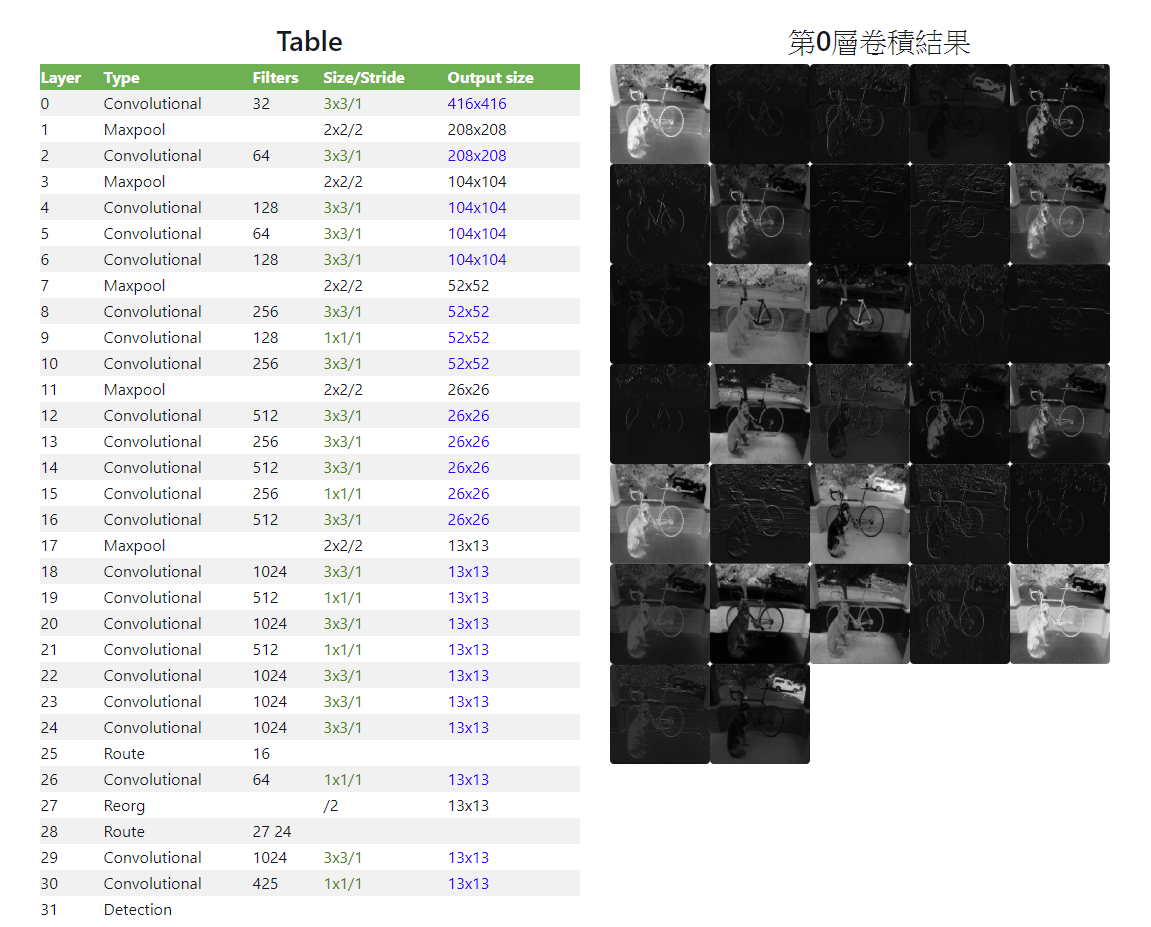
\includegraphics[width=0.5\textwidth]{fig/system1.png}
    \caption{\label{fig:系統1}系統示意圖.}
\end{figure}